\section{Eksperimendid}

Eksperimentide koostamiseks, mille abil uurida VMP ja BP algoritmide headust, on mitmeid viise. 

Esimesel juhul uurime $N$ mudelit ja andmestikku, mis on genereeritud võrdlemisi väikese $T \in \{10,15,20\}$ korral, et oleks mõistlikku ajaga võimalik läbi vaadata kõik võimalikud Viterbi rajad. Nii on võimalik täpselt leida,
\begin{itemize}
    \item kui kaugele optimumist on jäänud töös kirjeldatud algoritmidega leitud rajad logtõenäosuse vahena,
    \item mis on leitud rajade protsentiilid, ja
    \item tähtsa osana ka seda, kui kaugel on leitud rajad optimaalsest rajast Hammingu kauguse mõttes.
\end{itemize}
Kui Hammingu kaugus on enamasti väike, siis see annaks alust loota, et leides kõik rajad, mis on lähedal VMP ja BP abil leitud rajadele, on Viterbi rada nende hulgas. Veenvat teoreetilist põhjendust selle uskumiseks töö käigus ei otsitud, kuid suure $T$ korral on vaja mingit strateegiat heade kandidaatradade otsimiseks, sest ei ole realistlik leida tõenäosused kõigile $|\mathcal{X}|^T$ rajale nt $T=100$ korral. Toome siinkohal ka välja, et Hammingu ümbrust võib ka vaadata andmestiku genereerinud raja $x_1,\ldots,x_T$ korral, kuid on osutunud, et enamasti see rada on optimumist kaugel.

Vaatleme eksperimentides kaht mudelit. 

\subsection{Paarikaupa varjatud tunnusega Markovi ahel}

Esimene on paarikaupa varjatud tunnusega Markovi ahel (\ref{eq:model1_1}), (\ref{eq:model1_2}), (\ref{eq:model1_3}). Üleminekumaatriks on genereeritud Dirichlet' jaotusest parameetritega $1,\ldots,1$ ehk iga $u_{t-1},x_{t-1}$ korral on elemendiviisiliselt jaotus kirjeldatav kui
\begin{align}
    \label{eq:hmm1}
    p(u_t,x_t | u_{t-1},x_{t-1}) &\sim Cat(A_{u_{t-1},x_{t-1}}),& A_{u_{t-1},x_{t-1}} \sim Dir(1,\ldots,1)\\
    \label{eq:hmm2}
    p(u_1,x_1) &\sim Cat(A_1), &A_1 \sim Dir(1,\ldots,1) .
\end{align}
Emissiooni $y_t$ tiheduse määrab normaaljaotus keskväärtusega $x_t$ ning standardhälbega $1.25$ nagu ka \parencite{Soop.2023} eksperimentides, ehk 
\begin{equation}
    \label{eq:hmm3}
    p(y_t|x_t) = f_{\mathcal{N}}(y_t-x_t,1.25).
\end{equation}
Sellise mudeli puhul on võrdluseks kasutatud ka naiivset algoritmi, mis seab $x_t = \argmin |x_t - y_t|$.

\subsubsection{Eksperimendid väikese $T$ korral}

Uuritava mudeli korral on algoritmide tulemused paljulubavad ning paistavad üksteist komplementeerivat: $T=20,N=50$ korral oli näha, et $25$ juhul saavutab BP parema raja ning $16$ juhul VMP; $T=15,N=100$ korral oli BP algoritm $43$ juhul parem, VMP $35$ juhul parem.

\begin{figure}
\centering
\begin{subfigure}{.5\textwidth}
  \centering
  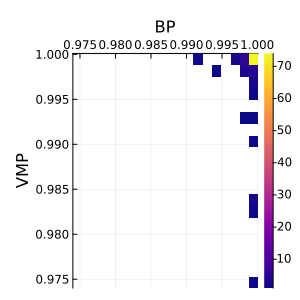
\includegraphics[width=1\linewidth]{uniform_dirichlet_percs_std125_t15.png}
  \caption{ $T = 15, N = 100$ }
  \label{fig:sub1}
\end{subfigure}%
\begin{subfigure}{.5\textwidth}
  \centering
  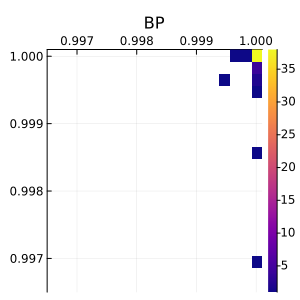
\includegraphics[width=1\linewidth]{uniform_dirichlet_percs_std125_t20.png}
  \caption{$T = 20, N = 50$}
  \label{fig:sub2}
\end{subfigure}
\caption{VMP ja BP algortimide protsentiilide kahedimensionaalne histogramm $N$ erineva katse mudeli (\ref{eq:hmm1}), (\ref{eq:hmm2}), (\ref{eq:hmm3}) korral. Graafikute teljed pole võrdsed.}
\label{fig:test}
\end{figure}

\begin{table}[!htb]
    \caption{Esimeses kolmes reas kujutame leitud radade tõenäosusi protsentiilidena ning viimases neljas radade Hammingu kauguseid optimumist.}
    \begin{subtable}{.5\linewidth}
      \centering
        \caption{$T = 15, N = 100$}
        \begin{tabular} {l|l l l l l}
\toprule
{} & {mean} & {min} & {max} \\ 
\midrule
\text{BP} & 0.9995 & 0.9919 & 1.0 \\
\text{VMP} & 0.9986 & 0.9746 & 1.0 \\
\text{ORIG} & 0.8851 & 0.09 & 0.9999 \\
\\
\text{H vmp} & 1.63 & 0.0 & 7.0 \\
\text{H bp} & 1.61 & 0.0 & 7.0 \\
\text{H orgin} & 5.22 & 1.0 & 12.0 \\
\text{H naive} & 2.68 & 0.0 & 8.0 \\
\bottomrule
\end{tabular}
    \end{subtable}%
    \begin{subtable}{.5\linewidth}
      \centering
        \caption{$T = 20, N = 50$}
        \begin{tabular}{l|l l l l l}
\toprule
{} & {mean} & {min} & {max} \\ 
\midrule
\text{BP} & 0.99997 & 0.99955 & 1.0 \\
\text{VMP} & 0.99986 & 0.99701 & 1.0 \\
\text{ORIG} & 0.92382 & 0.48647 & 0.9998 \\
\\
\text{H vmp} & 2.1 & 0.0 & 7.0 \\
\text{H bp} & 1.74 & 0.0 & 5.0 \\
\text{H orig} & 6.96 & 3.0 & 14.0 \\
\text{H naive} & 3.06 & 0.0 & 8.0 \\
\bottomrule
\end{tabular}
    \end{subtable} 
\end{table}

\subsection{Kolmekaupa Markovi ahel}

Teiseks kirjeldame kolmekaupa Markovi ahela (\ref{eq:model2_1}), (\ref{eq:model2_1}) eksperimente. Siin genereerisime samuti algtõenäosuste ja üleminekute maatriksid Dirichlet' jaotusest, kus iga $u_{t-1}, x_{t-1}, y_{t-1}$ korral on üleminek kirjeldatav kui
\begin{align*}
    p(u_t,x_t,y_t|u_{t-1},x_{t-1},y_{t-1}) &\sim Cat(A_{u_{t-1},x_{t-1},y_{t-1}}),& A_{u_{t-1},x_{t-1},y_{t-1}} \sim Dir(1,\ldots,1)\\
    p(u_1,x_1,y_1) &\sim Cat(A_1) ,& A_1 \sim Dir(1,\ldots,1)
\end{align*}

\subsubsection{Eksperimendid väikese $T$ korral}

BP tulemused on halvad. Uurin veel juhtu, kus BP saavutas halvima võimaliku raja. \bla

\begin{table}[!htb]
    \caption{Esimeses kolmes reas kujutame leitud radade tõenäosusi protsentiilidena ning viimases neljas radade Hammingu kauguseid optimumist.}
    \begin{subtable}{.5\linewidth}
      \centering
        \caption{$T = 15, N = 100$}
        \begin{tabular}{l|l l l l l}
\toprule
{} & {mean} & {min} & {max} \\ 
\midrule
\text{BP} & 0.97031 & 0.48843 & 1.0 \\
\text{VMP} & 0.96566 & 0.23636 & 1.0 \\
\text{ORIG} & 0.85045 & 0.13876 & 1.0 \\
& & & &\\
\text{H vmp} & 4.23 & 0.0 & 12.0 \\
\text{H bp} & 4.79 & 0.0 & 10.0 \\
\text{H orig} & 6.0 & 0.0 & 12.0 \\
\bottomrule
\end{tabular}
    \end{subtable}%
    \begin{subtable}{.5\linewidth}
      \centering
        \caption{$T = 20, N = 50$}
        \begin{tabular}{l|l l l l l}
\toprule
{} & {mean} & {min} & {max} \\ 
\midrule
\text{BP} & 0.8858 & 0.0 & 1.0 \\
\text{VMP} & 0.97881 & 0.59661 & 1.0 \\
\text{ORIG} & 0.83878 & 0.19275 & 0.99932 \\
& & & &\\
\text{H vmp} & 5.12 & 0.0 & 11.0 \\
\text{H bp} & 6.26 & 0.0 & 16.0 \\
\text{H orig} & 8.06 & 3.0 & 13.0 \\
\bottomrule
\end{tabular}
    \end{subtable} 
\end{table}

